
\begin{figure*}
	\centering
	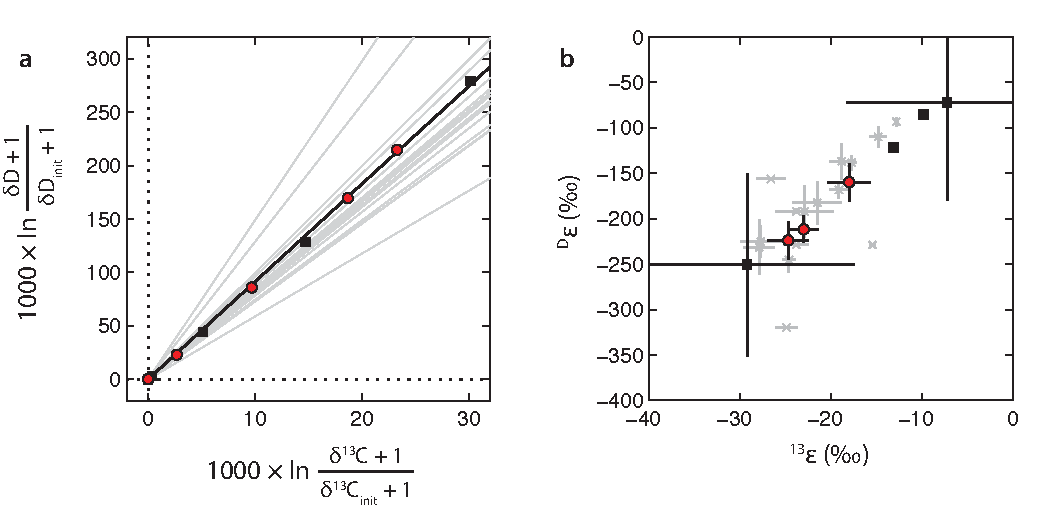
\includegraphics[width=0.95\textwidth]{figures/Fig4.2}
	\caption[\textsuperscript{13}C/\textsuperscript{12}C and D/H fractionation by aerobic methanotrophs]{Relationship between fractionation of carbon and
		hydrogen isotopes. \textbf{(a)} Data from the 30 and 37~°C experiments (\autoref{tab:4:1})
		are shown with black and red symbols, respectively. Black line (\emph{y}
		= 9.14 \emph{x}) represents the best-fit regression through the data.
		From \autoref{eqn:4:17}, the slope of this line is (\textsuperscript{D}$\alpha$ $-$
		1)/(\textsuperscript{13}$\alpha$ $-$ 1), or
		\textsuperscript{D}$\varepsilon$/\textsuperscript{13}$\varepsilon$. Near the origin, the
		\emph{x}- and \emph{y}-axes are approximately equal to
		δ\textsuperscript{13}C $-$ δ\textsuperscript{13}C\textsubscript{init} and
		δD $-$ δD\textsubscript{init}, respectively; this approximation becomes
		less accurate with increasing distance from the origin, particularly for
		hydrogen \parencite{Sessions+Hayes_2005_GCA}. Gray lines represent
		previously-reported correlations between fractionation of carbon and
		hydrogen isotopes by aerobic methanotrophs determined from experiments
		with pure cultures \parencite{Feisthauer++_2011_GCA} and enrichment cultures
		\parencite{Coleman++_1981_GCA,Kinnaman++_2007_GCA,Powelson++_2007_EST}.
		\textbf{(b)} Fractionation factors ($\varepsilon$, defined as $\alpha$ $-$ 1) calculated for
		individual bottle incubations from this study (\autoref{tab:4:1}) plotted against
		fractionation factors reported in the cited studies (gray). One point
		from the 37~°C experiment (41 h) was not plotted because of large
		uncertainties arising from a minimal extent of reaction.}
	\label{fig:4:2}
\end{figure*}